\documentclass{article}
\usepackage{arxiv}

\usepackage[utf8]{inputenc} % allow utf-8 input
\usepackage[T1]{fontenc}    % use 8-bit T1 fonts
\usepackage{hyperref}       % hyperlinks
\usepackage{url}            % simple URL typesetting
\usepackage{booktabs}       % professional-quality tables
\usepackage{amsfonts}       % blackboard math symbols
\usepackage{nicefrac}       % compact symbols for 1/2, etc.
\usepackage{microtype}      % microtypography
\usepackage{lipsum}
\usepackage{amsmath}
\usepackage{amsthm}
\usepackage{amsfonts}
\usepackage{enumerate}
\usepackage{setspace}
\usepackage{tkz-euclide}
\usepackage{graphicx}

\title{Shock wave in Traffic Flow Model}


\author{
  Huy Nguyen \\
  Department of Mathematics and Statistics\\
  Georgia State University\\
  %% examples of more authors
   \And
  Adam Nguyen \\
  Department of Mathematics and Statistics\\
  Georgia State University\\
   \And
  Simone Isom \\
  Department of Mathematics and Statistics\\
  Georgia State University\\
  \And
  Hieu Ngo \\
  Department of Mathematics and Statistics\\
  Georgia State University\\
  %% \And
  %% Coauthor \\
  %% Affiliation \\
  %% Address \\
  %% \texttt{email} \\
  %% \And
  %% Coauthor \\
  %% Affiliation \\
  %% Address \\
  %% \texttt{email} \\
}

\begin{document}
\maketitle

\begin{abstract}
The purpose is to combine a model predictive control (MPC) to predict the optimal speed for vehicles in a high density traffic. The concept of using time prediction method is to predict when the traffic will happen and reduce the congestion in traffic.
\end{abstract}



\section*{Introduction}
 Stuck in a intersection, you always watch unfold the Fundamental Problem of Traffic. On green, the first car accelerates, and then the next and then keep going until you only to catch the red. Had the car accelerate simultaneously, you would have made it through. Coordination, not cars is the problem. Human has slow reaction time and short attention spans. This dis-coordination limits how many cars can get through an intersection, and one backs up to the next, that's when city-sized gridlock cascades happen, taking forever to damp out. In general analysis, the more intersections, equal mores dis-coordination which equals more traffic congestion. This is the motive behind freeway, big highways: "No intersections". Theoretically, Even though there are splits and merges, but there is no stopping, no coordination problems, no traffic.
 
 
 However, intersection outside of a highway will back up onto it. Human reaction times limit how many cars can escape off-ramp when the light changes. Moreover, even without intersections, there would still be traffic on the highway. For example, take a one lane highway with a constant flow and moderate density, then all of a sudden an object cross the road. The driver sees it brakes a little, the following car brakes a little harder and the chain reaction keeps on going until someone reach a complete stop. In a multi-lane highway, there is no chicken. However, if a driver decided to change lanes rapidly with cars too close behind would be enough to birth one. Though the object is no longer be there, it left a phantom intersection on the highway, or we can understand at a shock wave point. "Shock waves are waves that originate from a sudden, substantial change in the state of the traffic flow. That is, a shock wave is defined by a discontinuity in the flow-density conditions in the time-space domain."
 
 By the properties, shock waves move. It's like a snake slithering down the road eating on coming cars and damp out the other end. Set up an experiment where cars with a moderate density and initiated velocity driving in a circle. As soon as one car has a different velocity than the initial velocity. This will start a shock wave of traffic that will last forever, even though there is no accident nor problem with the road, and cars. The solution for the problem is somehow, all the drivers coordinates and accelerate simultaneously, the shock wave will be eventually cease. 
 
 Therefore, as a driver, participate in a traffic, you have a high responsibility of causing traffic by your driving behavior. Always keeps the distance two cars from the car in front and behind you. Tailgating is a trouble since it is more likely to cause accident, or you as the tailgater can cause shock wave point if the driver ahead breaks. However, this will never be the solution for traffic congestion.
 
In traffic, the congestion will grow if the shock wave
travels faster than the damping point and vice versa. We as a group are seeking an optimization solution for this every day problem, a structural systematization solution. 

The METANET model was created as optimization formulation for macroscopic traffic flow problem and solved
using a genetic algorithm. The road networks are represented as directed graphs with nodes and links; the links are
homogeneous road sections with constant number of lanes and no changes to the curvature or gradients of the roads.
The links connect the nodes, and in turn, the nodes are used at places where the geometry of the motorway changes or
at the on-ramp or off-ramp junctions [10]. On the other hand, the model predictive control are able to solve the problem
of the optimal coordination of speed limits [2]. We use the METANET model to make predictions of the traffic and
apply the model predictive control (MPC) to find the optimal control inputs.
Therefore, as a driver participating in traffic, you have a high responsibility of causing traffic by your driving behavior.
Always keeps the distance two cars from the car in front and behind you. Tailgating instigates trouble since it is more
likely to cause accident, or you as the tailgater can cause shock wave point if the driver ahead breaks. However, this
will never be the solution for traffic congestion. In traffic, the congestion will grow if the shock wave travels faster than
the damping point and vice versa. We as a group are seeking an optimization solution for this every day problem, a
structural systematization solution.
\section*{METANET Model Overview}
We are using METANET Model as the fundamental solution. From there further dissect the disadvantage of METANET and optimize to become further more efficient.

METANET is a well known macroscopic traffic flow model.
A road network is represented as a directed graph consisting of nodes and links. Links represent homogeneous
road sections, where the number of lanes is a constant
and there is no significant change of curvature or gradient.
Nodes are connected by links and are used at places where
the geometry of the motorway changes or at on-/off-ramp
junctions. Traffic enters via origin links and leaves through
destination links. $$V[p_{m,i}(k)=v_{f,m}*exp[-\frac{1}{\alpha_{m}}(\frac{p_{m,i}(k)}{p_{cr,m}})^{\alpha_{m}}]$$

In which $p_{m,i}(k)$ is the traffic density, mean speed $v_{f,m}$,traffic volume or flow $q_{m,i}(k)$, and k indicates the time instant.

However,
    The METANET model does not describe the effect of speed limits.
     The dynamic equations are nonlinear. Then if the constraints of the control variable are not properly set up, it causes problems for the numerical optimization process.
     The density and ramp meter rate through density dynamics are tightly and non-linearly coupled with the speed control variables complicates the control design.
    The model cannot quickly identify significant changes in fast transition phases of traffic dynamics. 



\section*{Methods}
\label{sec:headings}

Our goal is to find an optimization solution for traffic conditions that produce shock wave. As previously discussed, shock waves are “waves that originate from a sudden, substantial change in the state of the traffic flow. A shock wave is defined by a discontinuity in the flow-density conditions in the time space domain. As a group we applied the model predictive control to optimally coordinate variable speed limits. The purpose of the control is to find the control signals that minimize the total time the vehicles spend in the network. 

We look back to the Fundamental Problem of Traffic. Every vehicles will enter the road from a pit with an initial velocity. At the connection point between the pit and the ring road, you set up a meter with a camera installed Model Predictive Control, and a speed limit prediction. We indicate that if each car cross the meter reach $v_1<v_0$, then the meter turn on the yellow signal. If the camera detects a complete stop on sight, then the meter turns on traffic control mode. Depends on the distance between the stopped car and the camera, the camera will determine the stop-and-go time for each vehicle such that the car exits out the shock wave point and will follow the speed $v_2$, until the last car has reach $v_2$. If the camera no longer detects congestion, the meter stops and $v_2$ change back to $v_1$ until the next shock wave point.

At each time step k, the optimal control signal is computed over a prediction horizon $N_p$. A control horizon $N_c$($< N_p$) is selected to reduce the number of variables and to improve the stability of the system. After the control horizon has been passed, the control signal is usually taken to be constant.  A rolling horizon strategy indicates that at each step, only the first sample of the optimal control signal is applied to the system. Afterwards, the time axis is shifted one sample step, we update the model and restart the procedure. This results in an on-line adaptive control scheme.

We modify the equation for the desired speed to incorporate speed limits and its effects. Another extension focuses on the modeling of the different nature of a mainstream origin as opposed to an on-ramp origin of the shock wave. We also consider the different effect of the downstream density gradient on speed when it is positive or negative. We see the effects of the speed limit by scaling down the desired speed by $v_{\text{ctrl}}/v_{\text{free},m}$. Then we can observe where the speed would be lower than the speed limit. Scaling down the speed limit also reduces the capacity of the road. However, these assumptions exaggerate the effects of the speed limits.
\section*{Optimization problem}
We want to apply the model predictive control to optimally coordinate variable speed limits. The purpose of the control is to find the control signals that minimize the total time the vehicles spend in the network. We want to predict the time that shock wave will occur with given certain density and traffic flow velocity. In this particular problem, We will also use Greenshield law of velocity. Greenshield was able to develop a model of uninterrupted traffic flow that predicts and explains the trends that are observed in real traffic flows. While Greenshield’s model is not perfect, it is fairly accurate and relatively simple. Greenshield made the assumption that, under uninterrupted flow conditions, speed and density are linearly related.

We also use Rankine-Hugoniot relations in order to solve the optimization problem. Despite Rankie-Hugoniot is broadly using in gas flow, we believe that this relation can apply for traffic aswell. In this particular problem, we only look at how properties of traffic would change across normal shock wave for density condition. The initial expression is $$\frac{\rho_{1}}{\rho_{2}}=\frac{(\gamma +1)M_{1}}{2+(\gamma -1)M_{1}}$$ This shows that the density ratio just depends on the Mach number $M_{1}$ of the flow up stream of the shockwave, and the ratio of the specific heats of the gas $\gamma$. Traffic has a similar condition where the problem only focus on the upstream value. However, gas and traffic have different movement, where gas contains molecules that will push each other to move forward, while with vehicles, at one congested point, we have to use drag force which relies a lot on acceleration. Traffic is simultaneous, we decided to use differential equation and partial derivative to further solve the problem replacing $\gamma$ and Mach number by $\epsilon$ and $\rho$


We first start with traffic flow equation $$\rho_{t}+C(\rho)\rho_{x}=0$$ and use Greenshield's Model to predict the ideal velocity that vehicle can go in a high density roadway. 

Finally, we have a piece-wise function 

\[ \begin{cases} 
      \rho_{L} & x \leq -\epsilon \\
      \rho_{L} + \frac{\rho_{R}-\rho_{L}}{2\epsilon}(x+\epsilon) & -\epsilon \leq x\leq \epsilon \\ 
      \rho_{R} & x \ge \epsilon 
   \end{cases}
\]

\noindent predicts the density of traffic. The condition to form a shockwave is $\rho_L < \rho_R$. As we can predict the time and the position when the shockwave forms, we can combine with MPC to optimize vehicle speed limit. 

Let C be the value of the vehicle speed and let $x_S^{(0)}, t_S^{(0)}$ be the position of the shock formation. 

There are 2 scenarios: 
\[ \begin{cases} 
      x=C_Lt - \epsilon & \text{for } C_L = C(\rho_L) \\
      x=C_Rt+ \epsilon & \text{for } C_R = C(\rho_R)
   \end{cases}
\]

$$C_L t_S^{(0)} - \epsilon = C_R t_S^{(0)} + \epsilon \text{: shock forms}$$

$$t_S^{(0)} = \frac{2\epsilon}{C_L-C_R} \text{ and } x_S^{(0)} = C_L t_S^{(0)} - \epsilon$$

$$x_S^{(0)} = \epsilon\left(\frac{C_L+C_R}{C_L-C_R}\right)$$

This creates a discontinuity. Using the Rankine-Hugoniot condition, 
$$\frac{d}{dt}x_S(t) = \frac{1}{2}(C_L+C_R)$$

When we simplify the equation, $$x_S(t) = \frac{1}{2}(C_L+C_R)t \text{ where } t > t_S^{(0)}$$


We want to use the Rankine-Hugoniot condition on Greenshield's Model to find the time value that vehicle will approach to shock wave point. We then use the time value to combine with model predictive control to optimally coordinate variable speed limit.


\section*{Set-up}

We debated between whether we use LIDAR ( Light Detection and Ranging ) or camera. Notice that LIDAR works better on analyzing the landscape rather than determine type of vehicles and counting problems, we decided to use camera. Most cameras you have seen on the road now, not only to indicate your speed limit, but also help the Department of Transportation determine the density and sort of the type of vehicle crossing each points, collecting data for future traffic infrastructure researches. 


For the setup, We first use cameras to indicate the density at a congestion point interval. In most heavy traffic point, they often have the infrastructure with the traffic light to go off ramp, traffic control box, etc. We will use the MPC algorithm to feed the traffic control box, so that
At the off-ramp meter, the light turns green for normal density, yellow light when there are higher density to indicate the drivers to be cautious of the cars around them. During rush hour, we apply the MPC algorithm to determine the stop time for exit ramp vehicles.
At the on-ramp traffic lights, during normal density, the MPC will prioritize vehicles ready to exit the roads and enter the freeway. When there are higher density of cars, the MPC will use traffic sensor to control traffic and moderate timing for traffic lights to avoid congestion at choke points. Finally, during rush hours, the MPC will prioritize vehicles moving in local roads to reduce the amounts of vehicle entering the freeway.

For data collection purpose, we use Cities : Skylines, the game developed by Colossal Order and Tantalus Media to run our experiment. Using traffic manager mods, we replicate the condition of 60 miles on I-75 I-285 intersection North and South Bound to further observe how traffic behave with and without Model Predictive Control. Our goal is without model predictive control, the data collect from the simulation can be as close as the real data provided from Georgia Department of Transportation. After the condition is perfect and the data without Model Predictive control matches with the real data, we further turn on MPC to process the data and compare to the original data.
\section*{Result}
We found that the optimal prediction horizon is approximately $N_p=10$ min. A control horizon $N_c=9$ min was necessary. When the difference $N_p-N_c$ is constant, an increase of $N_p$ causes a small decrease of the total time spent (TTS). In the controlled case, the shock wave disappears after approximately 1.5 hours, while in the no control case, the shock wave travels through the whole link. The active speed limits start to limit the flow at $t=10$ min and create a low density wave traveling downstream. The low density wave meets the upstream traveling shock wave and reduces its density and stops it.

The figures describe how many vehicles can go through a traffic point every hour in a day with and without Model Predictive Control. We assume the ideal condition where there are no crashes, no construction work, and people obey the speed limit while keeping lane changing to a minimum.The graph is the result from the simulation. The dark blue line represents the real data from
Georgia Department of Transportation at one location in I-75 [6]. The line represents the density of traffic through
that point every hour for a day. We picked up this intersection to simulate the situation due to its easy landscape and
generally uncrowded details; then we can show the effectiveness of vehicles on and off interstate highway. The blue line
is the data collect from the simulation with the identical condition. We had to bound the density of vehicles crossing the
point at 2800 vehicles/hour. The reason is that when you compute a linear regression of optimization in any traffic flow,
if the simulation perform significantly better than real data, it is hard to conclude that we can apply our method. If you
can restrict simulated data so that vehicles, weather, road, traffic lights, etc. can behave like real time, then the result
should be identical and less than 10 \% significant. Eventually, our goal is to let vehicles move away from shockwave
point and reach to the damping point faster, not more vehicles can go through traffic. The regression line only show that
at the same amount of time, there are more vehicles can escape traffics so that the traffic flow rate perform better with
our on-ramp or off-ramp control system. Without MPC, where the freeway speed limit is 55, 65, or 70 $m/h$, it will take each vehicle 15 to 20 minutes to travel to miles with the average speed under 25 $m/h$; additionally, the vehicles will take 37 to 44 minutes to traverse 5 miles with the average speed under 10 $m/h$. Now with the MPC in place, in the same scenarios, it will take 7 to 9 minutes to travel 2 miles with the average speed under 45 $m/h$ and 20 to 23 minutes to travel 5 to 7 miles with the average speed under 22.

\begin{figure}[ht]
    \centering
    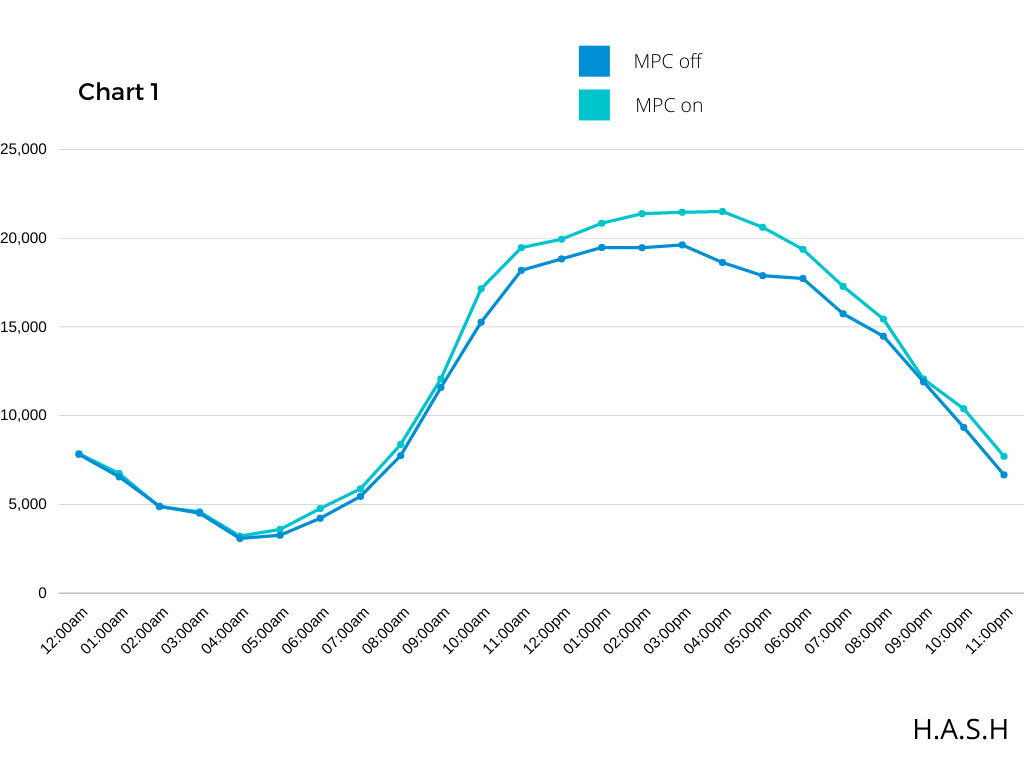
\includegraphics[width=100mm,scale=0.5]{Chart_1.png}
    
\end{figure}

These are non-practical results since we can only run in a simulator. The margin of error of the scenarios would be much closer if we apply it to real traffic. The results still stands in favor of the MPC model since there was a significant improvement in traffic congestion. 

We found that the MPC was able to solve traffic problem by reducing the time by approximately 20\% to 25\%. The system produces safety on the road by reducing the collision percentage since speed is moderated. 

The upstream "end" of the shock wave has a fixed location while the downstream "end" dissolves into free flow traffic in the uncontrolled situation. The shock wave eventually dissolves. In high density areas, the speed limits persist until the shock wave dissolves. The outflow after the shock wave entered the link is restored to earlier capacity in controlled case.



\section*{Discussion}

Cost and efficiency. The model is only an upgrade of what we have been using. For further improvement, we can change the stop exit signal to the actual stop meter where they have a stop timer and indicates what speed you should drive while participating in the interstate. We will re-program the traffic control box and connect them simultaneously so that the data will feed to the traffic control box faster from camera, and from traffic box control to traffic signals. The system is also easy to maintain since we can control remotely, diagnose and fix will be easier. The data will be exchange and transfer on a cloud base system so that it also could help parties which involves in navigation and data sciences to receive live data instead of satellites. 

In addition, it is efficiency such that high-density locations have already applied the equipment but only use very basic traffic sensors. Using this algorithm would improve our potential to control traffic. It is relatively cheaper and more affordable than other solutions. Due to low maintenance of the system, we can remotely control it by cloud base system. Finally, we can optimize or upgrade our algorithm, further can collect data, using AI to develop a better version of it.

Self-driving cars are the structurally systematized solution for this problem. Self-driving car can be programmed to stay in the middle of two vehicles and accelerate simultaneously. That is the fundamental idea to program a self-driving vehicle. The more self-driving cars participating on traffic, the more efficient the traffic flow gets. Professor Alex Bayen, Director of UC Berkeley proposed that when an automated car led human-controlled vehicles, stop-and-go traffic was eliminated and gas usage was reduced by 42\%.

The limitation we found is that the system cannot be use in roundabout traffic. While running the algorithm in one roundabout, the meter cannot indicate how long one car should stop since they cannot predict the direction of one vehicle moving. It causes even more traffic in moderate traffic conditions. There are also human factor. As long as people disobey the time and the speed assigned for each vehicle, the traffic will still be there if we speed up and do not keep a good distance with other vehicles. It won’t completely solve the traffic problem. Suppose there will always be traffic by a random phenomenon. Despite all the crashes, high density grows much faster than traffic flow, hence we can only reduce the time participated vehicles stuck in traffic rather than make traffic congestion disappear. 
\section*{Conclusion}
This paper presented the upgrade version of modeling road network METANET model. The resulting shows the slight improvement compared on what the system lacks, combining with Traffic flow function and model prediction to make MPC even more efficient. Our contribution is by using the Rankie-Hugoniot condition to find the initial time and position of given density to determine when the shock wave will form to further control traffic by using improved Model Predictive Control, prevent or “stretch” the flow rate so that the congestion point can damp out faster.
Although it has been almost a century since we first invented traffic signal, we tried to make it a better, more efficient traffic communicating tool but yet to achieve it. With this model, we look for a promising result that the coordination between traffic signals and drivers can improve. Eventually, traffic is and always will be for big cities, though we look forward to seeing a bright future where with better traffic communication, people will less likely stay hours stuck in traffic.
\section*{Acknowledgement}
The research was my idea, so that I helped people get into the problem as easy to understand as possible since this is a large topic to cover.

I am reponsible for the output of the research. I was able to find the expression of position and time of shock wave forms using Rankine-Hugoniot characteristic. My work is to run the simulation, fix the variables if the data did not match and observe whether the system have a potential in reality. I also contributed in mathematical optimization such as finding the partial derivatives of position $x$ and $t_{o}$ in Rankine-Hugoniot condition. 

Hieu is responsible for the outline and the structure of the presentation. Hieu helped us with related articles and find useful source to help the research as well as incorporating in the presentation

Adam and Hieu is responsible for METANET and MPC researches. He basically helped us understand how the model work, the advantages and disadvantages of the model, what we can do to further improve the model. Eventually because of his work, we were able to connect the relationship between METANET and our work to further execute our experiments.

Simone is responsible for the most part of the presentation, from wording, images. She also looks for different factors such as pollution and what this model is capable of to help G.A traffic is getting better. She also helps the group collecting data from Georgia Department of Transportation. Simone also helps Adam with the METANET and MPC researches.


Despite our individual works, we maintain assignments in which we have to work together, such as solving mathematical problem with given values. From our hypothesis result, we collect each other ideas to come up with the set-up, seeking of potential errors so that our set-up can be as easy and the most efficient result.
\section*{References}
\label{sec:headings}
\begin{enumerate}
    \item Adu, I. K., Boah, D. K., Tulasi, V. (2014). Application of System of Linear Equations to Traffic Flow for a Network of Four One-Way Streets in Kumasi, Ghana. \textit{International Journal of Contemporary Mathematical Sciences, 9} (14), 653-660. http://dx.doi.org/10.12988/ijcms.2014.410109 
    \item Breton, P., Hegyi, A., De Schutter, B., Hellendoorn, H. (2002). Shock wave elimination/reduction by optimal coordination of variable speed limits. \textit{Proceedings of the IEEE 5th International Conference on Intelligent Transportation Systems}, 225-230.
    \item Chapter 08: Shock Wave Analysis - TU Delft OCW”. TU Delft OCW, 2021, https://ocw.tudelft.nl/coursereadings/chapter8shockwaveanalysis/?courseid = 8959.
    \item De Vlieger, I., De Keukeleere, D., Kretzschmar, J. G. (2000). Environmental effects of driving behaviour and congestion related to passenger cars. Atmospheric Environment, 34(27), 4649–4655. https://doi.org/10.1016/s1352-2310(00)00217-x 
    \item GA DOT traffic density https://gdottrafficdata.drakewell.com/publicmultinodemap.asp 		http://www.dot.ga.gov/DS/Data
    \item Hofer, C., Jäger, G., Füllsack, M. (2018). Large scale simulation of CO2 emissions caused by Urban Car Traffic: An agent-based network approach. Journal of Cleaner Production, 183, 1–10. https://doi.org/10.1016/j.jclepro.2018.02.113 
    \item Lu, X.-Y., Qiu, T. Z., Horowitz, R., Chow, A., Shladover, S. (2011). METANET Model Improvement for Traffic Control. \textit{Conference Record - IEEE Conference on Intelligent Transportation Systems, 2} (2), 2148-2153. DOI:10.1109/ITSC.2011.6082936
    \item Mathew, T. V. (2019, January 10). Grade Seperated Intersection. Grade separated intersection. Retrieved November 1, 2021, from https://www.civil.iitb.ac.in/tvm/nptel/567Grade/web/web.html\#x1-40002.1. 
    \item Recurring traffic bottlenecks: A Primer focus on low-cost operational improvements (fourth edition). Recurring Traffic Bottlenecks (Fourth Edition) - Appendix C. Case Studies - FHWA Office of Operations. (n.d.). Retrieved November 1, 2021, from https://ops.fhwa.dot.gov/publications/fhwahop18013/appc.htm. 
    \item Poole, A., Kotsialos, A. (2016). Traffic Flow Model Validation Using METANET, ADOL-C and RPROP. \textit{IFAC-PapersOnLine, 49} (3), 291-296. 
    \item Williams, G. Traffic Flow. \textit{Advanced Engineering Mathematics 4th Edition}, 20-21.
    \item Alexandre M. Bayen. Eliminating Traffic Jams with Self-Driving Cars
\end{enumerate}


\end{document}

